% !TeX program = pdflatex
\documentclass[preprint,12pt]{elsarticle}

\usepackage[T1]{fontenc}
\usepackage[utf8]{inputenc}
\usepackage{amsmath,amssymb,amsthm,mathtools}
\usepackage{booktabs}
\usepackage{graphicx}
\graphicspath{{/mnt/data/}}
\usepackage{hyperref}
\usepackage{microtype}
\microtypesetup{expansion=false}
\usepackage{url}
\usepackage{adjustbox}
\usepackage{float}

\hypersetup{colorlinks=true,linkcolor=blue,citecolor=blue,urlcolor=blue}
\journal{Pattern Recognition Letters}

\newtheorem{proposition}{Proposition}

\newcommand{\R}{\mathbb{R}}
\newcommand{\node}{\mathcal{N}}
\newcommand{\calJ}{\mathcal{J}}
\newcommand{\calS}{\mathcal{S}}
\newcommand{\Imp}{I}
\newcommand{\gain}{G}
\newcommand{\n}{n}
\newcommand{\nL}{n_{\mathrm L}}
\newcommand{\nR}{n_{\mathrm R}}
\newcommand{\K}{K}

\begin{filecontents*}{references.bib}
@book{breiman1984cart,
  author    = {Leo Breiman and Jerome H. Friedman and Richard A. Olshen and Charles J. Stone},
  title     = {Classification and Regression Trees},
  publisher = {Wadsworth},
  address   = {Belmont, CA},
  year      = {1984}
}

@article{breiman2001rf,
  author  = {Leo Breiman},
  title   = {Random Forests},
  journal = {Machine Learning},
  volume  = {45},
  number  = {1},
  pages   = {5--32},
  year    = {2001},
  doi     = {10.1023/A:1010933404324}
}

@article{geurts2006extra,
  author  = {Pierre Geurts and Damien Ernst and Louis Wehenkel},
  title   = {Extremely Randomized Trees},
  journal = {Machine Learning},
  volume  = {63},
  number  = {1},
  pages   = {3--42},
  year    = {2006},
  doi     = {10.1007/s10994-006-6226-1}
}

@article{gilbertmosteller1966,
  author  = {John P. Gilbert and Frederick Mosteller},
  title   = {Recognizing the Maximum of a Sequence},
  journal = {Journal of the American Statistical Association},
  volume  = {61},
  number  = {313},
  pages   = {35--73},
  year    = {1966},
  doi     = {10.1080/01621459.1966.10502008}
}

@article{ferguson1989secretary,
  author  = {Thomas S. Ferguson},
  title   = {Who Solved the Secretary Problem?},
  journal = {Statistical Science},
  volume  = {4},
  number  = {3},
  pages   = {282--296},
  year    = {1989},
  doi     = {10.1214/ss/1177012493}
}

@inproceedings{nuti2023single,
  author    = {Pranav Nuti and Jan Vondr{\'a}k},
  title     = {Secretary Problems: The Power of a Single Sample},
  booktitle = {Proceedings of the 2023 ACM-SIAM Symposium on Discrete Algorithms},
  pages     = {2015--2029},
  year      = {2023},
  publisher = {SIAM},
  doi       = {10.1137/1.9781611977554.ch77}
}

@inproceedings{rubinstein2020samples,
  author    = {Aviad Rubinstein and Jack Z. Wang and S. Matthew Weinberg},
  title     = {Optimal Single-Choice Prophet Inequalities from Samples},
  booktitle = {11th Innovations in Theoretical Computer Science Conference (ITCS 2020)},
  series    = {LIPIcs},
  volume    = {151},
  pages     = {60:1--60:10},
  year      = {2020},
  publisher = {Schloss Dagstuhl -- Leibniz-Zentrum f{\"u}r Informatik},
  doi       = {10.4230/LIPIcs.ITCS.2020.60}
}

@article{samuelcahn1984,
  author  = {Ester Samuel-Cahn},
  title   = {Comparison of Threshold Stop Rules and Maximum for Independent Nonnegative Random Variables},
  journal = {The Annals of Probability},
  volume  = {12},
  number  = {4},
  pages   = {1213--1216},
  year    = {1984},
  doi     = {10.1214/aop/1176993150}
}

@article{laurentmassart2000,
  author  = {B{\'e}atrice Laurent and Pascal Massart},
  title   = {Adaptive Estimation of a Quadratic Functional by Model Selection},
  journal = {The Annals of Statistics},
  volume  = {28},
  number  = {5},
  pages   = {1302--1338},
  year    = {2000},
  doi     = {10.1214/aos/1015957395}
}

@article{romano2022pmlb,
  author  = {Joseph D. Romano and Trang T. Le and William La Cava and John T. Gregg and Daniel J. Goldberg and Natasha L. Ray and Praneel Chakraborty and Daniel Himmelstein and Weixuan Fu and Jason H. Moore},
  title   = {PMLB v1.0: an open-source dataset collection for benchmarking machine learning methods},
  journal = {Bioinformatics},
  volume  = {38},
  number  = {3},
  pages   = {878--880},
  year    = {2022},
  doi     = {10.1093/bioinformatics/btab665}
}
\end{filecontents*}

\begin{document}

\begin{frontmatter}

\title{Secretary-Style Split Search for Decision Trees}

\author[inst1]{Mathias Valla}
\address[inst1]{Chaire DIALog, Institut Louis Bachelier, Paris, France}

\begin{abstract}
The standard CART splitter examines all admissible covariate--threshold pairs at each node, which can make tree induction computationally expensive when many continuous features are available. This paper asks whether such exhaustive split enumeration is always necessary to grow accurate decision trees. We study a small family of secretary-style split-search rules that evaluate only a random subset of candidate splits and stop early according to simple sequential criteria. The proposed strategies include a single-stream secretary rule over random splits, a double secretary rule over covariates and thresholds, a covariate-level secretary rule with exhaustive within-covariate refinement, and a parametric secretary rule calibrated from exact gain evaluations. We also adapt the block-rank algorithm as a rank-adaptive secretary-style alternative.

The methods are compared with the standard exhaustive \texttt{scikit-learn} splitter and with ExtraTrees-style random-threshold baselines using several \texttt{max\_features} budgets, on a broad collection of regression and classification datasets from the PMLB benchmark suite. In regression, secretary rules are generally dominated by the random-threshold baselines, especially when the latter are allowed to inspect more features per node. In classification, conservative and rank-adaptive secretary variants remain competitive: covariate-level secretary and block-rank trade modest predictive loss for larger time savings, while one low-overhead parametric configuration is competitive on small classification datasets. Secretary-style split search is therefore best viewed as a conservative classification-time approximation rather than as a universal replacement for exhaustive or ExtraTrees-style split search.
\end{abstract}

\begin{keyword}
decision trees \sep CART \sep secretary problem \sep randomized split search \sep benchmark evaluation \sep computational efficiency
\end{keyword}

\end{frontmatter}

\section{Introduction}
\label{sec:introduction}

Classification and regression trees remain widely used for tabular data because they combine flexibility, interpretability, and strong empirical performance \cite{breiman1984cart}. Their standard induction rule is greedy: at each internal node, CART evaluates candidate covariate--threshold pairs and selects the split maximizing the impurity decrease. For continuous covariates, the number of admissible thresholds can be large, so exhaustive split search may dominate training time.

This raises a basic question: is it always necessary to evaluate all admissible splits in order to grow an accurate tree? In many nodes, only a small subset of candidates attains gains close to the optimum. Existing randomized tree procedures exploit this idea indirectly. Random forests subsample covariates \cite{breiman2001rf}, and extremely randomized trees randomize threshold choice \cite{geurts2006extra}. These methods, however, are not formulated as stopping rules on a stream of candidate gains.

We recast split search as a secretary-style online selection problem. In the classical secretary problem, items arrive sequentially in random order and the decision maker must stop online to select a highly ranked item \cite{gilbertmosteller1966,ferguson1989secretary}. The classical skip rule, with asymptotic success probability $1/e$, shows that a short exploration phase can be followed by a simple acceptance rule with a nontrivial guarantee \cite{gilbertmosteller1966,ferguson1989secretary}. More recent work has introduced rank-adaptive rules based on the availability of a single sample, including the block-rank family \cite{nuti2023single}. These ideas suggest a natural analogue for tree induction: if covariates and thresholds are explored in random order, split selection becomes a stopping problem on a stream of exact impurity gains.

We study four secretary-style split-search strategies for CART, ranging from direct split-level stopping to covariate-level stopping and model-based calibration, and also include a rank-adaptive block-rank variant and a one-sample prophet-style baseline.

The contribution is empirical and methodological rather than theoretical. We benchmark the proposed rules against the standard exhaustive \texttt{scikit-learn} splitter and against ExtraTrees-style random-threshold baselines on a large collection of regression and classification datasets from the PMLB benchmark suite \cite{romano2022pmlb}. The goal is to characterize the time--accuracy trade-off, quantify the variability induced by randomized split exploration, and identify which stopping rules offer the best practical compromise. An open-source implementation of all methods and the scripts used to reproduce the experiments are released publicly.\footnote{Code available at \href{https://github.com/MathiasValla/EarlyStoppingTrees}{https://github.com/MathiasValla/EarlyStoppingTrees}}

\section{Methods}
\label{sec:methods}

\subsection{Split-search setting}
\label{subsec:setup}

Consider a node $\node$ containing $\n$ observations $\{(X_i,Y_i)\}_{i=1}^{\n}$ with $X_i\in\R^p$. Let $\calJ=\{1,\dots,p\}$ be the set of covariates, and let $\calS_j$ be the set of admissible thresholds for covariate $j$. A candidate split is a pair $(j,s)$ with $s\in\calS_j$, producing children of sizes $(\nL,\nR)$. For an impurity $\Imp$, the gain of split $(j,s)$ is
\begin{equation}
\label{eq:generic_gain}
\gain_{j,s}
=
\Imp(\node)
-
\frac{\nL}{\n}\Imp(\node_L)
-
\frac{\nR}{\n}\Imp(\node_R).
\end{equation}
For regression, $\Imp$ is the mean squared error impurity. For classification, we consider Gini and entropy impurities \cite{breiman1984cart}. Once a threshold is sampled, its gain is computed exactly on the full node data. Randomness therefore comes only from the order in which covariates are visited and from random sampling of thresholds within covariates.

To study early stopping, we impose a random order on covariates and, within each visited covariate, a random order on thresholds. Split search then becomes a sequential decision problem on a stream of exact gains. In the experiments, the exploration budget at a node is parameterized as a function of node size $\n$, with schedules of order $\n/e$, $0.1\n$, $\log \n$, and $\sqrt{\n}$.

\subsection{Stopping rules}
\label{subsec:strategies}

Method $S$ treats split search as a single secretary problem over a random stream of candidate pairs $(j,s)$. Given a budget $B$, it rejects the first $r$ candidates and then accepts the first subsequent split whose gain exceeds all gains observed in the exploration phase. If no such split appears, the best candidate seen so far is returned. This is the direct adaptation of the classical secretary rule \cite{gilbertmosteller1966,ferguson1989secretary}.\\
\\
Method $S_{\mathrm{all}}$ applies the secretary rule at the covariate level. For a visited covariate $j$, its score is
\[
V_j=\max_{s\in\calS_j}\gain_{j,s}.
\]
Covariates are processed in random order, and a secretary rule is applied to the sequence $(V_j)$. When a covariate is accepted, the best threshold within that covariate is returned. This method is more expensive than $S$ for each inspected covariate, but it preserves exact within-covariate optimization.\\
\\
Method $S^2$ introduces a nested secretary structure. The outer rule is applied to covariates in random order. For each visited covariate $j$, an inner secretary rule is applied to a random threshold stream inside $\calS_j$. The inner rule returns a threshold $\hat s_j$ and a realized gain $\tilde V_j=\gain_{j,\hat s_j}$, and the outer rule is then applied to the sequence $(\tilde V_j)$. The outer stage selects the covariate and the inner stage selects the threshold.\\
\\
Method $S_{\mathrm{par}}$ is a model-based variant. For a given covariate $j$, a small number of random thresholds is first evaluated exactly, yielding gain samples used to fit a working distributional model. A stopping threshold is then derived from this fitted distribution, for example through a high quantile, and thresholds are sampled until one exceeds the fitted acceptance level. The goal is not to claim an exact generative law for random-threshold gains, but to provide a calibrated stopping rule based on a small number of exact evaluations.\\
\\
The block-rank algorithm replaces the single exploration threshold of the classical secretary rule by a sequence of rank-based thresholds that become more permissive across successive budget blocks \cite{nuti2023single}. In the present context, this yields a rank-adaptive stopping rule on a random stream of split gains. We evaluate it as a structured alternative to the simple secretary baseline.\\
\\
We also include a one-sample prophet-style baseline. For each covariate, one random threshold is sampled and evaluated exactly, and the maximum of these gains is used as an empirical acceptance threshold. A second pass then considers new random split candidates in random order and accepts the first one whose gain exceeds this threshold. This baseline is motivated by prophet inequalities from samples \cite{rubinstein2020samples,samuelcahn1984}.

\subsection{Motivating heuristics}
\label{subsec:theory}

This subsection is motivational only. We do not attempt a formal analysis of tree induction under secretary-style exploration, and the paper's contribution remains empirical and methodological.

The classical secretary problem shows that, under a random arrival order, a simple skip-then-accept rule with exploration length of order $N/e$ is asymptotically optimal for selecting the best item \cite{gilbertmosteller1966,ferguson1989secretary}. This is the only theoretical fact used directly in the benchmark design: it motivates the default $n/e$ exploration schedule that we treat as the representative secretary-style setting in the main comparison.

The parametric variant $S_{\mathrm{par}}$ was motivated more loosely. For a fixed split, regression gains under MSE admit an exact positive-valued law, whereas classification gains are often well approximated by chi-square- or gamma-like families under standard asymptotics. This suggests that a small sample of exact gain evaluations might be used to fit a working distribution and derive a conservative acceptance threshold \cite{laurentmassart2000}. In the present paper, however, this idea is used only as a heuristic calibration device; we do not claim that the fitted model is exact, nor do we derive guarantees for the resulting stopping rule.

All methods were implemented in a common open-source package built around a modified tree splitter, with identical tree-growing hyperparameters across methods. This ensures that the observed differences are attributable to split-search rules rather than to other changes in the induction procedure.

\section{Results}
\label{sec:results}

\subsection{Experimental protocol}
\label{subsec:protocol}

We compared secretary-style split search against the standard exhaustive splitter of \texttt{scikit-learn} and against ExtraTrees-style random-threshold baselines with \texttt{max\_features} set to \(1\), \(p/3\), \(2p/3\), and \(p\), on a broad collection of regression and classification datasets from the PMLB benchmark suite \cite{romano2022pmlb}. For each dataset, the same 5-fold cross-validation splits and tree hyperparameters were used across methods. Because the proposed procedures are randomized, each dataset--method pair was evaluated over 100 independent runs with different estimator seeds. One classification dataset succeeded under one impurity criterion but not the other, so the Gini and entropy comparisons reported in the paper were restricted to the common set of 119 datasets that ran successfully under both criteria.

The primary computational metric is wall-clock training time. To make the timing results more interpretable, we also track split-search effort through the number of gain evaluations, either measured directly for the secretary-style splitters or reconstructed deterministically a posteriori for the exhaustive and ExtraTrees baselines. Predictive performance is measured by RMSE in regression and by F1-score in classification; accuracy, effort plots, and additional visualizations are reported in the supplementary material. Results are normalized relative to the exhaustive splitter through a speedup factor and a relative loss metric.

\begin{table}[t]
\centering
\caption{Summary of the PMLB benchmark used in the study.}
\label{tab:datasets}
\begin{adjustbox}{max width=\textwidth}
\begin{tabular}{lrrrrr}
\toprule
Task & $N$ & Median $n$ & Median $p$ & $n_{\min}$--$n_{\max}$ & $p_{\min}$--$p_{\max}$ \\
\midrule
Regression & 107 & 500 & 10 & 47--40768 & 2--124 \\
Classification (Gini) & 119 & 675 & 13 & 32--58000 & 2--216 \\
Classification (Entropy) & 119 & 675 & 13 & 32--58000 & 2--216 \\
\bottomrule
\end{tabular}
\end{adjustbox}
\end{table}


\subsection{Global trade-off}
\label{subsec:main_results}

Figure~\ref{fig:pareto_main} summarizes the main Pareto comparison between speedup and predictive degradation. Each point corresponds to one dataset summarized by the median over the 100 runs. Size-stratified versions of the same Pareto comparison are reported in Supplementary Figure~S1. Three conclusions are immediate: all secretary-style rules save computation; the time--accuracy trade-off depends strongly on the task; and covariate-level and rank-adaptive rules are systematically safer than aggressive split-level secretary rules.

\begin{figure}[H]
\centering
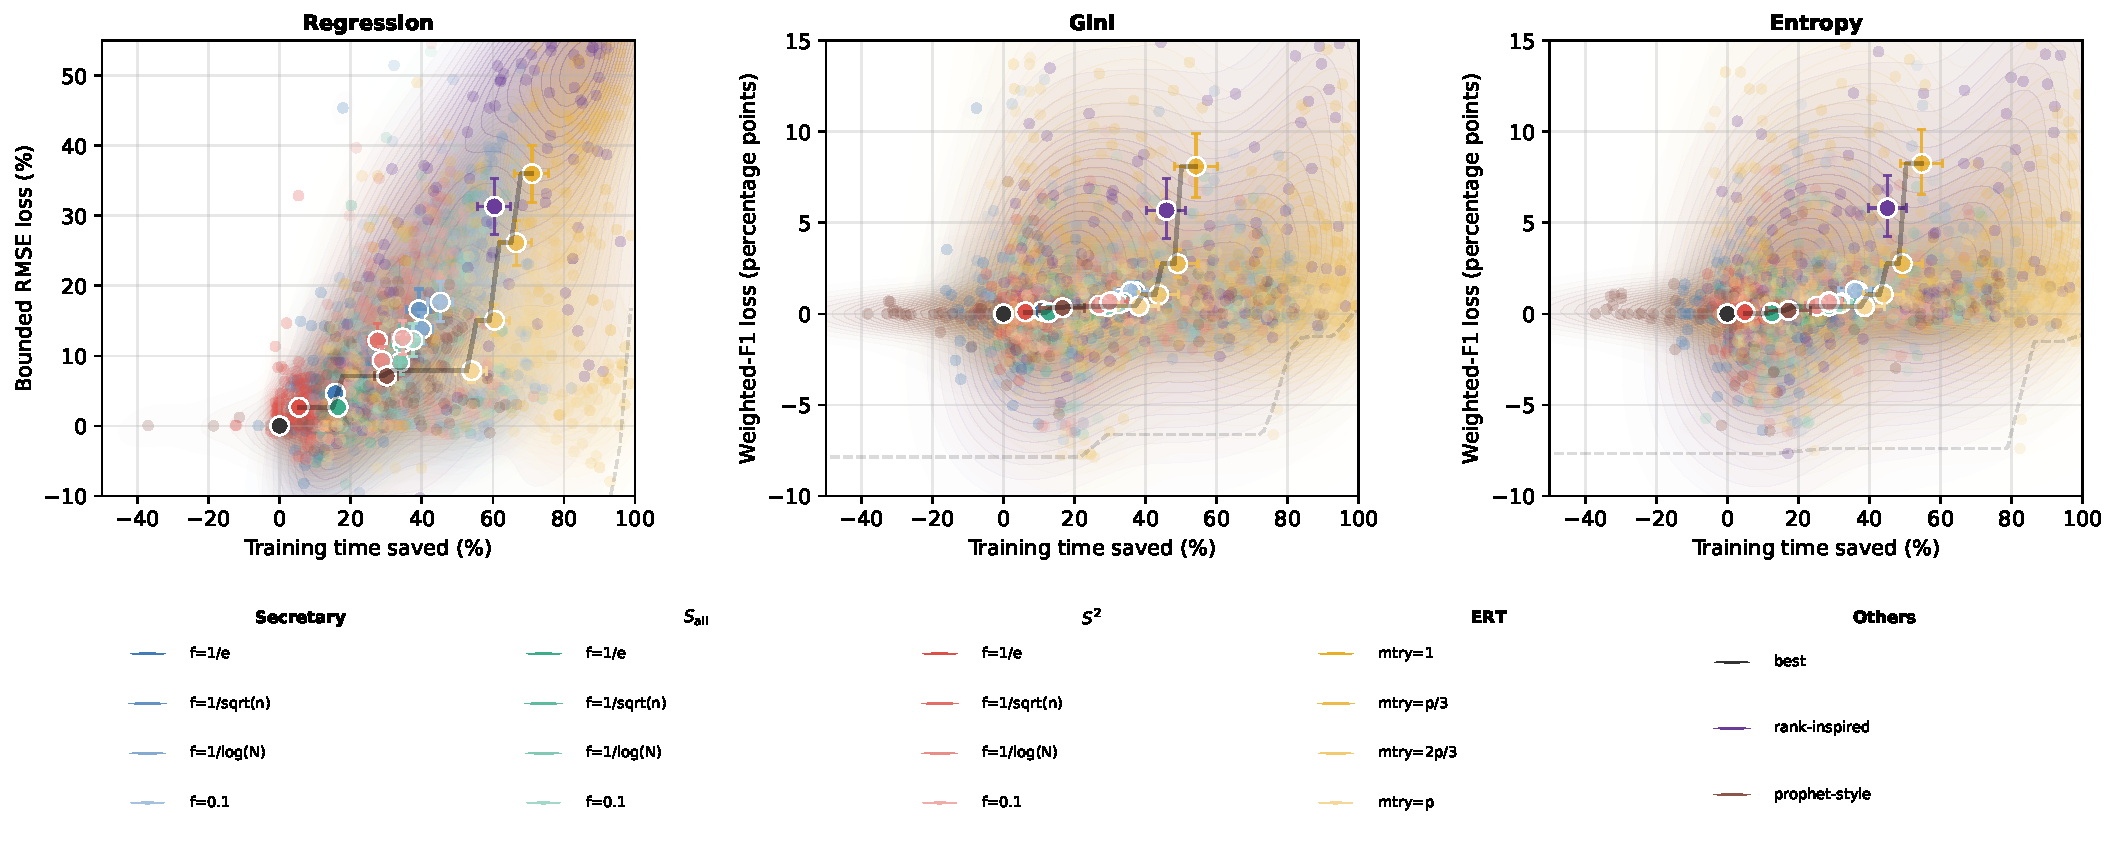
\includegraphics[width=1\linewidth]{MAIN_FIGURES/figure1_pareto_all.png}
\caption{Global Pareto comparison of exhaustive, secretary-style, and ExtraTrees-style split-search methods. Each point represents one dataset summarized by the median over 100 runs. The horizontal axis reports the median percentage of training time saved relative to the exhaustive \texttt{scikit-learn} splitter, and the vertical axis reports the median percentage loss relative to the same baseline. Left: regression with RMSE loss. Middle: classification with Gini impurity and F1 loss. Right: classification with entropy impurity and F1 loss. Large white-edged markers indicate the cross-dataset medians of the corresponding methods.}
\label{fig:pareto_main}
\end{figure}

Table~\ref{tab:summary_results} reports a representative benchmark summary. For the secretary families, we use the theoretically motivated $n/e$ schedule; for the parametric strategy, we report the low-overhead classification configuration \((10, q=0.5)\); and for ExtraTrees we report all four \texttt{max\_features} budgets. The table reports median speedup, median loss, 90th percentile loss, and two practical probabilities: the fraction of datasets for which the median loss remains below 5\%, and the fraction for which the median speedup is at least 20\%.


\begin{table}[t]
\centering
\caption{Representative global summary by method. The $n/e$ schedule is used for the secretary families, the low-overhead \((10,q=0.5)\) configuration is used for \(S_{\mathrm{par}}\) in classification, and all four ExtraTrees \texttt{max\_features} budgets are shown. Speedup is relative to the exhaustive \texttt{scikit-learn} splitter. Loss is expressed in percent. Full results for all schedules are reported in the supplementary material.}
\label{tab:summary_results}
\begin{adjustbox}{max width=\textwidth}
\begin{tabular}{llrrrrr}
\toprule
Task & Method & Median speedup & Median loss (\%) & 90th pct.\ loss (\%) & $P(\mathrm{loss}\le 5\%)$ & $P(\mathrm{speedup}\ge 20\%)$ \\
\midrule
Regression & Exhaustive & 1.00 & 0.0 & 0.0 & 1.000 & 0.000 \\
Regression & $S$ ($n/e$) & 7.45 & 42.0 & 58.0 & 0.086 & 1.000 \\
Regression & $S^2$ ($n/e$) & 2.05 & 36.1 & 57.6 & 0.159 & 0.947 \\
Regression & $S_{\mathrm{all}}$ ($n/e$) & 2.16 & 20.4 & 48.7 & 0.204 & 0.858 \\
Regression & Block-rank & 6.88 & 38.7 & 56.3 & 0.048 & 1.000 \\
Regression & 1-sample prophet & 2.69 & 23.9 & 57.1 & 0.095 & 0.990 \\
Regression & ExtraTree ($m_{\mathrm{try}}=1$) & 5.16 & 36.7 & 60.6 & 0.115 & 0.982 \\
Regression & ExtraTree ($m_{\mathrm{try}}=p/3$) & 4.08 & 28.4 & 44.5 & 0.150 & 0.956 \\
Regression & ExtraTree ($m_{\mathrm{try}}=2p/3$) & 3.25 & 15.2 & 29.0 & 0.221 & 0.938 \\
Regression & ExtraTree ($m_{\mathrm{try}}=p$) & 2.53 & 8.5 & 16.3 & 0.354 & 0.885 \\
\midrule
Classification (Gini) & Exhaustive & 1.00 & 0.0 & 0.0 & 1.000 & 0.000 \\
Classification (Gini) & $S$ ($n/e$) & 3.75 & 11.3 & 47.7 & 0.381 & 1.000 \\
Classification (Gini) & $S^2$ ($n/e$) & 1.62 & 4.8 & 40.2 & 0.508 & 0.885 \\
Classification (Gini) & $S_{\mathrm{all}}$ ($n/e$) & 1.66 & 1.6 & 10.8 & 0.770 & 0.836 \\
Classification (Gini) & $S_{\mathrm{par}}$ \((10,q=0.5)\) & 2.00 & 3.4 & 29.8 & 0.576 & 0.890 \\
Classification (Gini) & Block-rank & 3.64 & 5.2 & 24.7 & 0.500 & 1.000 \\
Classification (Gini) & 1-sample prophet & 2.22 & 7.5 & 26.3 & 0.424 & 0.890 \\
Classification (Gini) & ExtraTree ($m_{\mathrm{try}}=1$) & 2.29 & 4.6 & 21.9 & 0.525 & 0.951 \\
Classification (Gini) & ExtraTree ($m_{\mathrm{try}}=p/3$) & 1.97 & 1.7 & 7.9 & 0.779 & 0.934 \\
Classification (Gini) & ExtraTree ($m_{\mathrm{try}}=2p/3$) & 1.66 & 1.0 & 3.8 & 0.934 & 0.877 \\
Classification (Gini) & ExtraTree ($m_{\mathrm{try}}=p$) & 1.43 & 0.3 & 2.6 & 0.967 & 0.779 \\
\midrule
Classification (Entropy) & Exhaustive & 1.00 & 0.0 & 0.0 & 1.000 & 0.000 \\
Classification (Entropy) & $S$ ($n/e$) & 3.66 & 11.2 & 48.3 & 0.373 & 1.000 \\
Classification (Entropy) & $S^2$ ($n/e$) & 1.58 & 4.6 & 42.0 & 0.508 & 0.934 \\
Classification (Entropy) & $S_{\mathrm{all}}$ ($n/e$) & 1.62 & 1.7 & 10.5 & 0.754 & 0.877 \\
Classification (Entropy) & $S_{\mathrm{par}}$ \((10,q=0.5)\) & 1.97 & 3.8 & 29.5 & 0.534 & 0.873 \\
Classification (Entropy) & Block-rank & 3.66 & 5.0 & 25.9 & 0.500 & 1.000 \\
Classification (Entropy) & 1-sample prophet & 2.13 & 6.0 & 24.3 & 0.475 & 0.890 \\
Classification (Entropy) & ExtraTree ($m_{\mathrm{try}}=1$) & 2.29 & 4.4 & 21.9 & 0.516 & 0.951 \\
Classification (Entropy) & ExtraTree ($m_{\mathrm{try}}=p/3$) & 1.95 & 1.8 & 7.7 & 0.779 & 0.943 \\
Classification (Entropy) & ExtraTree ($m_{\mathrm{try}}=2p/3$) & 1.68 & 1.1 & 3.9 & 0.951 & 0.918 \\
Classification (Entropy) & ExtraTree ($m_{\mathrm{try}}=p$) & 1.49 & 0.5 & 2.3 & 0.975 & 0.820 \\
\bottomrule
\end{tabular}
\end{adjustbox}
\end{table}

The regression results are unfavorable to secretary-style approximation. The secretary rules save time, but they are dominated by the random-threshold baselines once those baselines are allowed to inspect more than one feature per node. In particular, \(\mathrm{ExtraTree}(m_{\mathrm{try}}=p)\) achieves median speedup \(2.53\times\) with median RMSE loss 8.5\%, whereas the best secretary-style compromise, \(S_{\mathrm{all}}(n/e)\), still incurs 20.4\% median loss at \(2.16\times\) speedup. Aggressive split-level rules such as \(S\), \(S^2\), and block-rank are faster, but their regression losses remain too large for the trade-off to be broadly attractive.

The classification results are more favorable, but they also show that the practical baseline set matters. The strongest global compromises are often achieved by ExtraTrees-style random-threshold search: with either Gini or entropy, \(\mathrm{ExtraTree}(m_{\mathrm{try}}=p/3)\) and \(\mathrm{ExtraTree}(m_{\mathrm{try}}=2p/3)\) keep median loss around 1--2\% while still delivering \(1.7\times\) to \(2.0\times\) speedups. Among the secretary-style rules, \(S_{\mathrm{all}}(n/e)\) and block-rank remain the most competitive: \(S_{\mathrm{all}}(n/e)\) matches the low-loss regime of the stronger ExtraTrees baselines, while block-rank trades larger loss for substantially larger speedups around \(3.6\times\). The screened parametric representative \(S_{\mathrm{par}}(10,q=0.5)\) reaches about \(2.0\times\) speedup with median loss 3.4--3.8\%, and Supplementary Figure~S2 shows that this configuration is mainly interesting on small classification datasets. By contrast, \(S\) and \(S^2\) are faster but substantially less reliable, with median losses near or above 5\% for \(S^2\) and above 11\% for \(S\).

A plausible explanation for the strong task asymmetry observed in the benchmark is that classification impurities are more tolerant to approximate split search than regression impurity. For Gini and entropy, many nearby thresholds can induce very similar child class proportions and therefore nearly equivalent impurity reductions. In such cases, partial random exploration may still identify a split whose downstream predictive effect is close to that of the exhaustive optimum. By contrast, regression gains based on MSE appear to depend more sharply on the precise threshold location, because small changes in the partition can alter child means and variances continuously and hence affect the final predictions more directly. Supplementary Figure~S13 examines this interpretation directly under exhaustive search by comparing the mass of thresholds within 5\% and 10\% of the nodewise optimum, the gap between the best gain and the median random-threshold gain, and the width of the near-optimal region on the winning covariate. The resulting comparison is more nuanced than a single scalar notion of flatness: some diagnostics are larger for regression, whereas the best-versus-random gap is larger for classification. This suggests that the empirical advantage of classification is not explained by one universal notion of broader near-optimal threshold regions alone, and likely reflects a combination of impurity geometry, competition across covariates, and downstream loss sensitivity.

\subsection{Reliability and dataset structure}
\label{subsec:reliability}

Figure~\ref{fig:reliability} complements the median-based summaries by showing reliability under explicit operating constraints. Aggressive methods such as $S$ and $S^2$ can satisfy moderate loss tolerances on a non-negligible subset of runs, especially in classification, but they also exhibit heavier tails of poor outcomes. Size-stratified reliability curves are reported in Supplementary Figure~S6, and the full grid of joint success probabilities over all datasets is reported in Supplementary Figure~S7.

\begin{figure}[H]
\centering
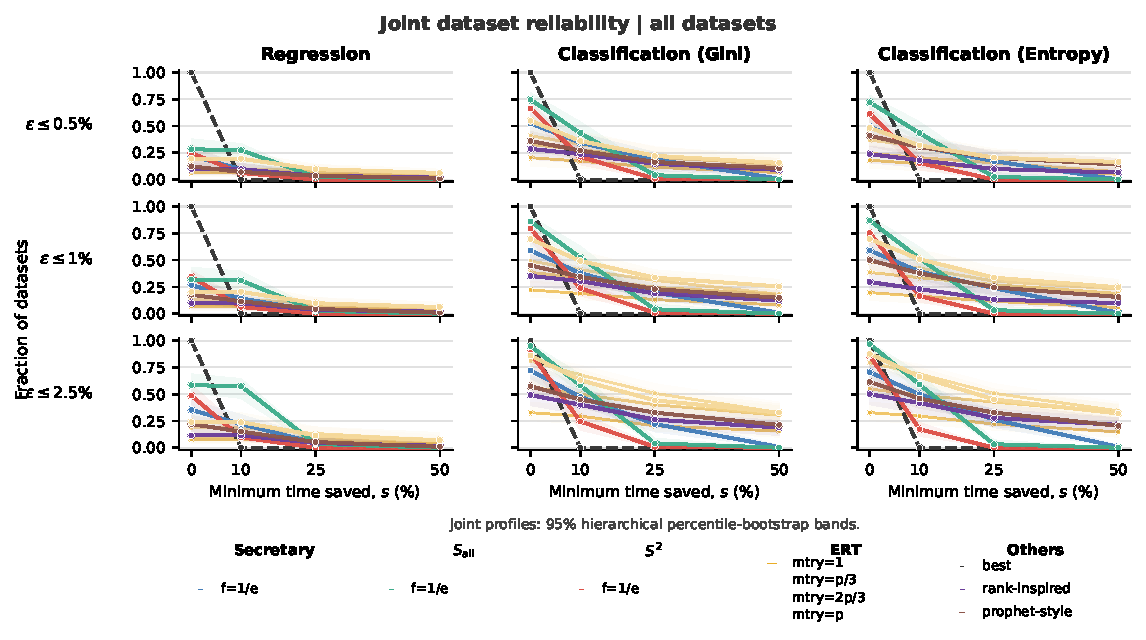
\includegraphics[width=1\linewidth]{MAIN_FIGURES/figure4_success_combined.png}
\caption{Reliability summaries for secretary-style split-search methods. Top row: empirical probability of achieving a predictive loss below a tolerance \(\varepsilon\). Bottom panels: empirical probability of simultaneously achieving at least a prescribed time saving and a predictive loss below a prescribed tolerance. Separate panels are shown for regression, classification with Gini impurity, and classification with entropy impurity. Size-stratified and method-specific variants are reported in the supplementary material.}
\label{fig:reliability}
\end{figure}

By contrast, $S_{\mathrm{all}}$ and block-rank are less aggressive but more reliable. This explains why $S$ and $S^2$ can appear competitive under permissive thresholds while still performing poorly in dataset-level medians. Their occasional strong runs do not compensate for their broader and more skewed loss distributions. Supplementary Figures~S3--S5 report task-specific ridgeline summaries of within-dataset variability, and Supplementary Figures~S9--S11 provide complementary whisker summaries of the same repeated-run variability.

\begin{figure}[H]
\centering
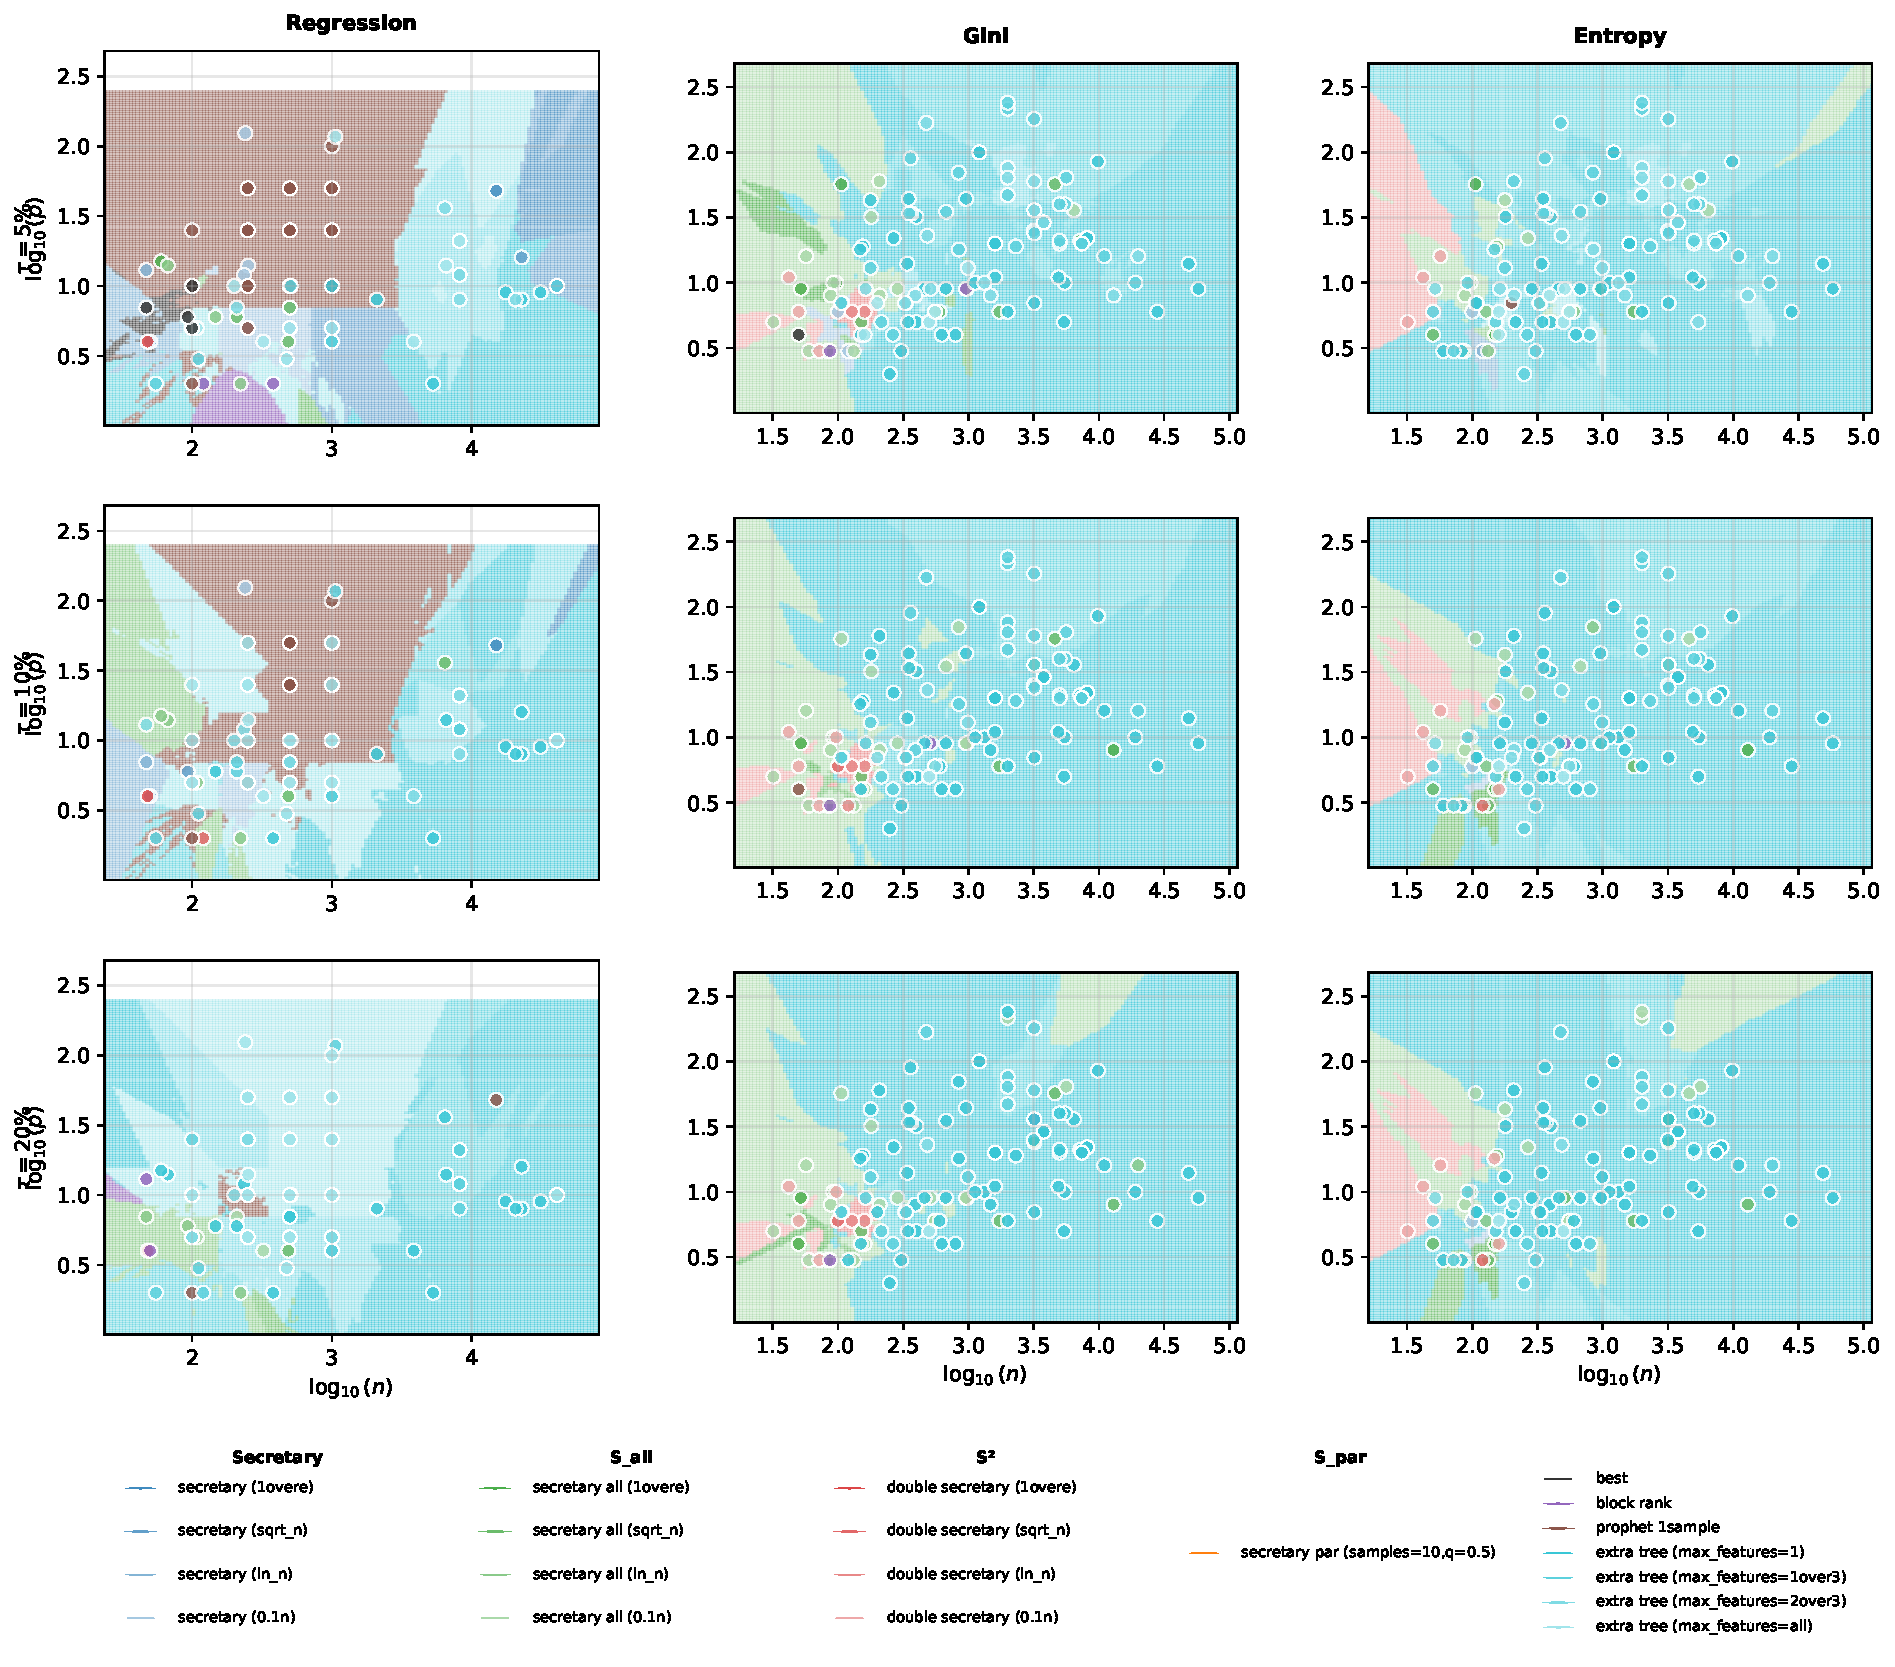
\includegraphics[width=1\linewidth]{MAIN_FIGURES/figure3_regime_combined.png}
\caption{Regime maps as a function of dataset size and dimensionality. Each point is a benchmark dataset represented in the \((\log_{10} n,\log_{10} p)\) plane and colored by the split-search strategy that gives the best practical trade-off under a fixed speedup--loss criterion. Columns correspond to loss tolerances \(\tau=5\%,10\%,20\%\). Rows correspond to regression, classification with Gini impurity, and classification with entropy impurity.}
\label{fig:dataset_structure}
\end{figure}

Figure~\ref{fig:dataset_structure} shows that the usefulness of secretary-style split search depends on dataset structure. Classification tasks are clearly more favorable than regression tasks. Within classification, and under the chosen speedup–loss criterion, covariate-level and rank-adaptive methods dominate larger portions of the regime map than split-level secretary rules. In regression, exhaustive split search remains the safest choice on much of the benchmark, and secretary-style rules are only competitive in limited regions.

\subsection{Sensitivity and negative result for the parametric strategy}
\label{subsec:ablation}

We examined four exploration schedules based on node size: $\n/e$, $0.1\n$, $\log \n$, and $\sqrt{\n}$. The full results are reported in the supplementary material. Changing the schedule affects the quantitative trade-off more than the qualitative ranking. For $S$ and $S^2$, more aggressive schedules produce slightly larger speedups at the price of slightly worse predictive degradation. For $S_{\mathrm{all}}$, the $n/e$ schedule consistently provides the best compromise, especially in classification, which justifies its use as the default representative in the main text. The corresponding size-stratified Pareto analyses, reliability summaries, and effort comparisons are reported in Supplementary Figures~S1, S6, S7, S14, and S15.

The parametric secretary method $S_{\mathrm{par}}$ was evaluated in an initial screening study over a grid of fitting sample sizes and quantile levels. Most configurations are dominated in practice: the cost of fitting the working model outweighs any benefit from early stopping, especially in regression and on larger classification datasets. One low-overhead classification configuration, however, remains competitive on small datasets, which is why we retain \(S_{\mathrm{par}}(10,q=0.5)\) as a representative line in the main classification figures and table. Even there, its global performance remains less robust than the strongest ExtraTrees, \(S_{\mathrm{all}}\), and block-rank baselines. This mostly negative result shows that probabilistic calibration is not useful by itself when the fitting overhead is too large relative to the gain-computation cost. \\
\\
For orientation, the supplementary material is organized as follows: Supplementary Figure~S1 gives the size-stratified Pareto comparison; Supplementary Figure~S2 gives the $S_{\mathrm{par}}$ screening study; Supplementary Figures~S3--S5 give the ridgeline summaries; Supplementary Figures~S6--S7 and~S12 give the reliability and joint-success plots; Supplementary Figure~S8 gives the regime maps; Supplementary Figures~S9--S11 give the within-dataset whisker summaries; Supplementary Figure~S13 gives exhaustive gain-landscape diagnostics for the regression--classification asymmetry; and Supplementary Figures~S14--S15 compare split-search effort across methods and against wall-clock savings.

\section{Conclusion, limitations, and outlook}
\label{sec:conclusion}

This paper asked whether exhaustive CART split search can be replaced, at least in part, by secretary-style sequential selection without incurring an unacceptable loss in predictive performance. The answer depends strongly on both the stopping rule and the prediction task. Secretary-style split search does reduce training time, sometimes substantially, but aggressive split-level strategies such as simple secretary and double secretary often do so at too high a predictive cost. More conservative or more structured variants remain practically competitive. In particular, the covariate-level strategy $S_{\mathrm{all}}$ and the rank-adaptive block-rank rule emerge as the most convincing compromises, especially in classification, where they provide meaningful speedups with comparatively modest degradation in predictive performance.

The study reveals a clear task asymmetry. Regression trees are much less tolerant to incomplete split exploration than classification trees. On the regression benchmarks considered here, even the best secretary-style variants remain far from the exhaustive splitter in predictive preservation. In classification, by contrast, the losses are often moderate enough to make the time--accuracy trade-off practically interesting. This suggests that the value of approximate split search depends on the impurity criterion and on the sensitivity of the task to local split errors.

A second important outcome is mostly negative but informative. The parametric secretary variant $S_{\mathrm{par}}$, although statistically motivated by gain-distribution approximations, is not competitive globally once fitting overhead is taken into account. One low-overhead configuration remains interesting on small classification datasets, but overall the family is less robust than the strongest ExtraTrees, \(S_{\mathrm{all}}\), and block-rank baselines. This cautions against assuming that a principled probabilistic calibration will automatically lead to an effective split-search procedure.

The study is limited to single trees, benchmark datasets, and a deliberately small family of stopping rules, and is intended primarily as an empirical characterization rather than a complete theory.

A natural next step is to study the same split-search rules in bagging and boosting. Because split-search cost is incurred at every node and across many trees, even moderate node-level savings may accumulate into substantial end-to-end gains. At the same time, ensembling may reduce the predictive effect of occasional suboptimal splits, which could make secretary-style rules more attractive than they are in single trees. A second direction is methodological: the performance of the block-rank rule suggests that adaptive rank-based or sample-based stopping rules may be preferable to the classical secretary rule in this context. Overall, secretary-style split search is not a universal replacement for exhaustive CART search, but in favorable settings, especially in classification, it offers a simple and interpretable way to trade split-search time against predictive performance.

\bibliographystyle{elsarticle-num}
\bibliography{references}

\end{document}
